% hyperbolas mucm = const in the (E, E') plane
\begin{center}
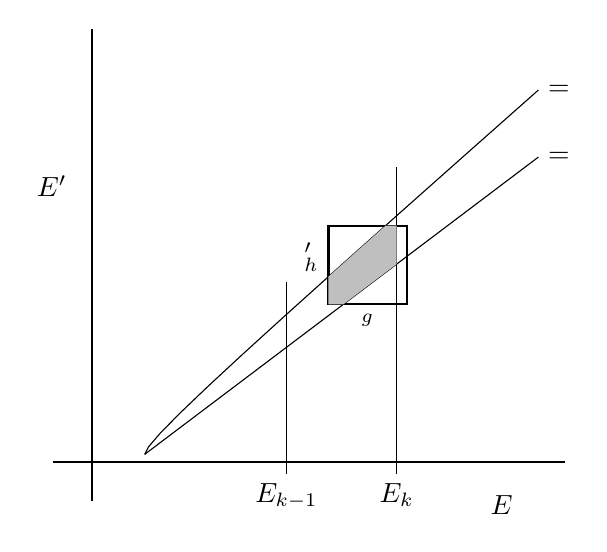
\begin{tikzpicture}
% the axes
  \draw[thick] (3.5,0) -- (10, 0);
  \draw[thick] (4,-0.5) -- (4, 5.5);
% the integration box
  \draw[thick](7,2) -- (7, 3) -- (8, 3) -- (8, 2) -- cycle;
% the data lines
  \draw (6.46667, -0.15) -- (6.46667, 2.28995);
  \node [below] at (6.46667, -0.15) {$E_{k-1}$};
  \draw (7.86667, -0.15) -- (7.86667, 3.74029);
  \node [below] at (7.86667, -0.15) {$E_{k}$};
% the curves
% mucm: -1
%\draw(4.66667, 0.0952381) --
%(4.71667, 0.0140642) --
%(4.86667, 0.00464791) --
%(5.11667, 0.0634261) --
%(5.46667, 0.187176) --
%(5.91667, 0.373109) --
%(6.46667, 0.618893) --
%(7.11667, 0.922636) --
%(7.86667, 1.28284) --
%(8.71667, 1.69832) --
%(9.66667, 2.16816);
% mucm: -0.5
%\draw(4.66667, 0.0952381) --
%(4.71667, 0.0735287) --
%(4.86667, 0.125453) --
%(5.11667, 0.24923) --
%(5.46667, 0.443248) --
%(5.91667, 0.706112) --
%(6.46667, 1.03666) --
%(7.11667, 1.43394) --
%(7.86667, 1.8972) --
%(8.71667, 2.42586) --
%(9.66667, 3.01946);
% mucm: 0
\draw(4.66667, 0.0952381) --
(9.66667, 3.87075);
% mucm: 0.5
\draw(4.66667, 0.0952381) --
(4.71667, 0.192458) --
(4.86667, 0.367064) --
(5.11667, 0.620838) --
(5.46667, 0.955391) --
(5.91667, 1.37212) --
(6.46667, 1.87219) --
(7.11667, 2.45654) --
(7.86667, 3.12593) --
(8.71667, 3.88094) --
(9.66667, 4.72204);
% mucm: 1
%\draw(4.66667, 0.0952381) --
%(4.71667, 0.251922) --
%(4.86667, 0.487869) --
%(5.11667, 0.806642) --
%(5.46667, 1.21146) --
%(5.91667, 1.70512) --
%(6.46667, 2.28995) --
%(7.11667, 2.96784) --
%(7.86667, 3.74029) --
%(8.71667, 4.60848) --
%(9.66667, 5.57333);
% integration region
\fill[gray!50] (7, 2) -- (7.0, 2.3517) -- 
(7.11667, 2.4565) -- (7.7256, 3) --
(7.86667, 3) -- (7.86667, 2.5116) --
(7.1892, 2) -- cycle;
% labels
 \node [below] at (9.2, -0.3) {$E$};
 \node [left] at (3.8, 3.5) {$E'$};
% \node [right] at (9.66667, 2.16816){$\mucm = -1$};
% \node [right] at (9.66667, 3.01946){$\mucm = -1/2$};
 \node [right] at (9.66667, 3.87075){$\mucm = \mucmjm$};
 \node [right] at (9.66667, 4.72204){$\mucm = \mucmj$};
% \node [right] at (9.66667, 5.57333){$\mucm = 1$};
 \node [left] at (7, 2.6){$\calE_h'$};
 \node [below] at  (7.5, 2){$\calE_g$};
\end{tikzpicture}
\caption{Integration region in the incident energy bin~$\calE_g$ and outgoing bin~$\calE_h'$
for probability data given at incident energies $E_{k-1}$ and~$E_k$ and direction
cosines $\mucmjm$ and~$\mucmj$ shown in the laboratory frame}
\label{Fig:2-body-region-lab}
\end{center} 
